\documentclass[11pt,letterpaper]{article}

% ── Packages ────────────────────────────────────────────────────────────────
\usepackage[margin=1in]{geometry}
\usepackage{amsmath,amssymb,amsthm}
\usepackage{mathtools}
\usepackage{algorithm}
\usepackage{algpseudocode}
\usepackage{booktabs}
\usepackage{array}
\usepackage{graphicx}
\usepackage{subcaption}
\usepackage{hyperref}
\usepackage{cleveref}
\usepackage{natbib}
\usepackage{microtype}
\usepackage{xcolor}
\usepackage{enumitem}
\usepackage{float}

% ── Theorem environments ─────────────────────────────────────────────────────
\newtheorem{theorem}{Theorem}[section]
\newtheorem{proposition}[theorem]{Proposition}
\newtheorem{remark}[theorem]{Remark}
\newtheorem{definition}[theorem]{Definition}

% ── Operators / macros ───────────────────────────────────────────────────────
\DeclareMathOperator{\E}{\mathbb{E}}
\DeclareMathOperator{\argmin}{arg\,min}
\newcommand{\bm}[1]{\boldsymbol{#1}}
\newcommand{\R}{\mathbb{R}}
\newcommand{\calQ}{\mathcal{Q}}
\newcommand{\calF}{\mathcal{F}}
\newcommand{\diag}{\mathrm{diag}}

% ── Title block ──────────────────────────────────────────────────────────────
\title{%
  \textbf{Stochastic Dual Dynamic Programming vs.\ Actor-Critic\\[4pt]
  Reinforcement Learning for Hydrothermal Scheduling:\\[4pt]
  A Comparative Study on the Brazilian Interconnected Power System}
}
\author{%
  ISEN 637 --- Stochastic and Dynamic Programming\\[4pt]
  \small Spring 2026
}
\date{}

% ─────────────────────────────────────────────────────────────────────────────
\begin{document}
\maketitle

\begin{abstract}
We compare two fundamentally different paradigms for solving the Brazilian
interconnected hydrothermal scheduling problem over a 24-month planning horizon:
Stochastic Dual Dynamic Programming (SDDP) and the Advantage Actor-Critic (A2C)
deep reinforcement learning algorithm.
SDDP exploits the linear, convex structure of the problem by iteratively
constructing piecewise-linear outer approximations of the Bellman cost-to-go
functions, guaranteeing convergence to the optimal policy on the discretised
scenario tree.
A2C treats scheduling as a Markov decision process and learns a parameterised
Gaussian policy via policy-gradient methods, guided by SDDP demonstrations
through behavioral cloning and a mixed imitation--RL loss with annealed BC weight.
Both methods operate on the same 4-subsystem aggregate model of the Brazilian
system, featuring a PAR(1) multiplicative inflow process, 95 thermal generating
units, four-level load curtailment penalties, and inter-regional energy exchange
through a transshipment hub.
The SDDP solution provides a provable lower bound against which the A2C policy is
benchmarked.
We analyse convergence behaviour, policy quality, computational cost, and the
effectiveness of warm-starting the neural policy from SDDP trajectories.
\end{abstract}

\tableofcontents
\clearpage

% ══════════════════════════════════════════════════════════════════════════════
\section{Introduction}
\label{sec:intro}
% ══════════════════════════════════════════════════════════════════════════════

The hydrothermal generation scheduling problem is one of the canonical large-scale
multistage stochastic optimisation problems in power systems operations.
Brazil's National Interconnected System (SIN) is particularly challenging:
approximately 75\% of installed capacity is hydroelectric, reservoir storage spans
multiple years, and inflows are highly seasonal and spatially correlated across
four major hydrological regions.
The system operator must decide, one month at a time over a multi-year horizon,
how much water to release from each reservoir for generation, how much thermal
capacity to dispatch, and how much energy to exchange between regions---all before
the next inflow realisation is observed.

Since the 1980s, the standard industrial solution has been Stochastic Dual Dynamic
Programming (SDDP)~\citep{pereira1991,shapiro2013}.
SDDP is a sampling-based approximate dynamic programming method that constructs a
lower approximation of the Bellman cost-to-go functions as a collection of
supporting hyperplanes (Benders cuts).
Because each stage subproblem is a linear program, the method scales to the
hundreds of stages and thousands of variables present in the full operational
planning problem.
Its convergence properties are well understood~\citep{philpott2008}, and it is
used operationally by the Brazilian grid operator ONS~\citep{shapiro2011}.

Deep reinforcement learning (RL) has recently emerged as an alternative for
operational planning under uncertainty.
Policy-gradient methods such as A2C~\citep{mnih2016} make no assumptions about
the convexity or differentiability of the system dynamics, and can in principle
handle nonlinear constraints, complex state representations, and end-to-end
learned dispatch heuristics.
However, they require large amounts of experience, exhibit high gradient variance,
and provide no optimality guarantees.

This paper conducts a rigorous head-to-head comparison of both methods on the same
24-month aggregate Brazilian model.
Our main contributions are:
\begin{enumerate}[noitemsep]
  \item A faithful implementation of the PAR(1) inflow model and the
        hydrothermal scheduling LP as an SDDP instance in Julia/\texttt{SDDP.jl}.
  \item An A2C agent with a 144-dimensional continuous action space, trained via a
        behavioral cloning (BC) warm-start on SDDP-generated demonstrations
        followed by mixed BC+RL fine-tuning with annealed imitation weight.
  \item A rigorous evaluation on 100 shared inflow scenarios, quantifying the
        optimality gap of the A2C policy relative to the SDDP policy cost and the
        SDDP lower bound.
  \item An analysis of the warm-start mechanism and the role of SDDP demonstrations
        in accelerating and stabilising A2C training.
\end{enumerate}

The remainder is organised as follows.
\Cref{sec:problem} defines the hydrothermal scheduling problem.
\Cref{sec:sddp} presents the SDDP algorithm.
\Cref{sec:a2c} develops the A2C formulation and BC warm-start.
\Cref{sec:experiments} describes the experimental setup.
\Cref{sec:results} presents and analyses the results.
\Cref{sec:discussion} discusses implications and limitations.
\Cref{sec:conclusion} concludes.

% ══════════════════════════════════════════════════════════════════════════════
\section{Problem Formulation}
\label{sec:problem}
% ══════════════════════════════════════════════════════════════════════════════

\subsection{System Description}
\label{sec:system}

Following~\citet{shapiro2013}, the Brazilian system is represented by an aggregate
model with four energy-equivalent reservoir nodes---Southeast (SE), South (S),
Northeast (NE), and North (N)---and one transshipment hub (Imperatriz, IM) that
mediates inter-regional energy exchange.
Each node aggregates all hydroelectric plants in its hydrological region into a
single equivalent reservoir with monthly regulation capacity.
The planning horizon is $T = 24$ months.

\paragraph{State variables.}
At stage $t \in \{1,\ldots,T\}$ the system state is:
\begin{itemize}[noitemsep]
  \item $v_{it} \in [0, \bar{v}_i]$: stored energy in reservoir $i \in \{1,2,3,4\}$
        (MWmonth), with upper bounds $\bar{v}_i$.
  \item $a_{it} \in [0, \infty)$: realised inflow to reservoir $i$, augmented as
        a state variable to handle the PAR(1) serial dependence.
\end{itemize}

\paragraph{Decision variables.}
At each stage the planner chooses:
\begin{itemize}[noitemsep]
  \item $q_{it} \in [0, \bar{q}_i]$: hydro generation at node $i$.
  \item $s_{it} \ge 0$: spillage from reservoir $i$.
  \item $g_{uit} \in [\underline{g}_{ui}, \bar{g}_{ui}]$: generation of thermal
        unit $u$ in region $i$.  There are $U = 95$ thermal units distributed as
        43 (SE), 17 (S), 33 (NE), 2 (N).
  \item $d_{ijt} \in [0, \delta_j L_{it}]$: energy deficit in subsystem $i$ at
        curtailment depth $j \in \{1,2,3,4\}$, where
        $\delta_j \in \{0.05,\, 0.05,\, 0.10,\, 0.80\}$.
  \item $e_{ijt} \in [0, \bar{e}_{ij}]$: energy flow from node $i$ to node $j$
        ($5 \times 5$ matrix including the IM hub).
\end{itemize}
The total decision dimension per stage is $4 + 4 + 95 + 16 + 25 = 144$.

\paragraph{Operational constraints.}
The following constraints must hold at every stage $t$:
\begin{align}
  &\textbf{Hydro balance:} &
  v_{i,t} + s_{it} + q_{it} &= v_{i,t-1} + a_{it},
  \quad i=1,\ldots,4, \label{eq:hydro_balance}\\[4pt]
  &\textbf{Power balance:} &
  \sum_u g_{uit} + q_{it} + \sum_j e_{jit} - \sum_j e_{ijt}
  + \sum_j d_{ijt} &= L_{it},
  \quad i=1,\ldots,4, \label{eq:power_balance}\\[4pt]
  &\textbf{Transshipment:} &
  \sum_{i=1}^{4} e_{i5,t} &= \sum_{i=1}^{4} e_{5i,t}, \label{eq:transshipment}\\[4pt]
  &\textbf{Variable bounds:} &
  \eqref{eq:bounds} \text{ as specified above.} \label{eq:bounds}
\end{align}
The monthly demand $L_{it}$ is deterministic with 12-period seasonality.
Complete recourse is ensured because the full demand can always be met by deficit.

\paragraph{Stage cost.}
\begin{equation}
  c_t(x_t) = \underbrace{\sum_{i=1}^{4}\sum_{u} c^{\mathrm{th}}_{ui}\,g_{uit}}_{\text{thermal}}
            + \underbrace{\sum_{i=1}^{4}\sum_{j=1}^{4} c^d_j\,d_{ijt}}_{\text{deficit}}
            + \underbrace{\sum_{i=1}^{5}\sum_{j=1}^{5} c^e_{ij}\,e_{ijt}}_{\text{exchange}}
            + \underbrace{c^s \textstyle\sum_{i=1}^{4} s_{it}}_{\text{spillage}},
  \label{eq:stage_cost}
\end{equation}
where unit thermal costs $c^{\mathrm{th}}_{ui}$ are taken from engineering data,
deficit penalties are $c^d \in \{1142.80,\; 2465.40,\; 5152.46,\; 5845.54\}$ (R\$/MWmonth)
increasing with curtailment depth, exchange costs $c^e_{ij}$ are small ($\le 0.001$),
and the spillage penalty is $c^s = 0.001$.

\subsection{Stochastic Inflow Model (PAR(1))}
\label{sec:inflow}

Following~\citet{shapiro2013}, monthly inflows are modelled by a Periodic
AutoRegressive process of order 1 (PAR(1)) with multiplicative log-normal errors.
Let $X_{it}$ denote the natural inflow to reservoir $i$ in month $t$,
$\hat{\mu}_{im}$ the sample log-mean for calendar month $m = ((t-1)\bmod 12)+1$,
and $\gamma_{im}$ the monthly autoregressive coefficient.
The model is:
\begin{equation}
  X_{it} = \varepsilon_{it}\!\left(
    e^{\hat{\mu}_{im}}
    + \gamma_{im}\,\frac{e^{\hat{\mu}_{im}}}{e^{\hat{\mu}_{i,m-1}}}
    \!\left(X_{i,t-1} - e^{\hat{\mu}_{i,m-1}}\right)
  \right),
  \label{eq:par1}
\end{equation}
where $\bm{\varepsilon}_t = e^{\bm{\eta}_t}$ with
$\bm{\eta}_t \sim \mathcal{N}(\mathbf{0}, \Sigma_m)$ iid across stages,
giving $\E[\bm{\varepsilon}_t] = \mathbf{1}$ (mean-one multiplicative error).
Raw noise samples are clamped to $\pm 3$ standard deviations before
exponentiation for numerical stability.

\paragraph{Linearised affine form.}
Model~\eqref{eq:par1} is not linear in $X_{i,t-1}$ due to the product
with $\varepsilon_{it}$.  The PAR(1) can be written exactly as:
\begin{equation}
  X_{it} = \underbrace{-\varepsilon_{it}\,\gamma_{im}\,
            \frac{e^{\hat{\mu}_{im}}}{e^{\hat{\mu}_{i,m-1}}}}_{\alpha_{it}}
            \cdot X_{i,t-1}
            + \underbrace{\varepsilon_{it}\,(1-\gamma_{im})\,e^{\hat{\mu}_{im}}}_{\beta_{it}}.
  \label{eq:par1_linear}
\end{equation}
Defining the noise vector $\omega_t = (\bm{\alpha}_t, \bm{\beta}_t) \in \R^8$,
the inflow update takes the affine form:
\begin{equation}
  X_{it} + \alpha_{it}\,X_{i,t-1} = \beta_{it},
  \label{eq:inflow_sddp}
\end{equation}
which is linear in the state variable $X_{i,t-1}$ for fixed $\omega_t$.
By augmenting the state with $a_{it} \coloneqq X_{it}$, the noise $\omega_t$
becomes independent of $a_{i,t-1}$ given $a_{i,t-1}$, satisfying the
\emph{stagewise-independence} condition required by SDDP.

\subsection{Multistage Stochastic Program}
\label{sec:msp}

The hydrothermal scheduling problem is a multistage stochastic linear program:
\begin{equation}
  \min_{x_1 \in \mathcal{X}_1}\; c_1^\top x_1 +
  \E_{\omega_2}\!\left[\min_{x_2 \in \mathcal{X}_2(x_1,\omega_2)}\; c_2^\top x_2 +
  \cdots +
  \E_{\omega_T}\!\left[\min_{x_T \in \mathcal{X}_T(x_{T-1},\omega_T)}\; c_T^\top x_T
  \right]\cdots\right],
  \label{eq:msp}
\end{equation}
where $x_t = (q_t, s_t, g_t, d_t, e_t)$ collects stage-$t$ decisions,
$\mathcal{X}_t(x_{t-1},\omega_t)$ encodes constraints~\eqref{eq:hydro_balance}--\eqref{eq:bounds},
and the objective is minimisation of expected total cost over 24 months.

% ══════════════════════════════════════════════════════════════════════════════
\section{Stochastic Dual Dynamic Programming}
\label{sec:sddp}
% ══════════════════════════════════════════════════════════════════════════════

\subsection{Algorithm Overview}

SDDP~\citep{pereira1991} solves problem~\eqref{eq:msp} by iteratively building
piecewise-linear outer approximations of the Bellman cost-to-go functions
$Q_t : \R^{n_{t-1}} \to \R$, defined by the backward recursion:
\begin{equation}
  Q_t(x_{t-1}) = \E_{\omega_t}\!\left[
  \min_{x_t \in \mathcal{X}_t(x_{t-1},\omega_t)} c_t^\top x_t + Q_{t+1}(x_t)
  \right],
  \quad Q_{T+1} \equiv 0.
  \label{eq:bellman}
\end{equation}
The current approximation at stage $t$ is the pointwise maximum over a collection
of supporting hyperplanes (cuts):
\begin{equation}
  \hat{Q}_t(x_{t-1}) = \max_{k \in \mathcal{I}_t}
  \left\{\alpha_{tk} + \beta_{tk}^\top x_{t-1}\right\} \le Q_t(x_{t-1}),
  \label{eq:cut_approx}
\end{equation}
where inequality holds because each cut is a supporting plane of the convex
function $Q_t$.  Because $\hat{Q}_t \le Q_t$, the stage-1 optimal value with
$\hat{Q}_2$ substituted is a \emph{lower bound} on the optimal value
of~\eqref{eq:msp}.

\paragraph{Forward pass.}
At each iteration, $M$ sample scenarios $\{\omega_t^{(j)}\}_{t=2}^T$ are drawn.
For each scenario $j$, the following LP is solved forward from $t=1$ to $t=T$:
\begin{equation}
  \bar{x}_t^{(j)} = \argmin_{x_t,\,\theta_{t+1}}
  \left\{c_t^\top x_t + \theta_{t+1} :
  x_t \in \mathcal{X}_t(\bar{x}_{t-1}^{(j)},\omega_t^{(j)}),\;
  \theta_{t+1} \ge \hat{Q}_{t+1}\right\}.
  \label{eq:forward_lp}
\end{equation}
The trial solutions $\bar{x}_t^{(j)}$ are stored for the backward pass.

\paragraph{Backward pass.}
Starting from $t = T$ and proceeding to $t = 2$, for each trial point
$\bar{x}_{t-1}$, the $N_t$ recourse subproblems (one per noise sample
$\omega_t^{(1)},\ldots,\omega_t^{(N_t)}$) are solved:
\begin{equation}
  Q_{t}^{(j)}(\bar{x}_{t-1}) = \min_{x_t,\,\theta_{t+1}}
  \left\{c_t^\top x_t + \theta_{t+1} :
  x_t \in \mathcal{X}_t(\bar{x}_{t-1},\omega_t^{(j)}),\;
  \theta_{t+1} \ge \hat{Q}_{t+1}\right\}.
  \label{eq:backward_lp}
\end{equation}
Let $\pi_t^{(j)}$ be the dual multiplier corresponding to the constraint
$B_t \bar{x}_{t-1} + A_t x_t = b_t^{(j)}$ in~\eqref{eq:backward_lp}.
A new Benders cut is appended:
\begin{equation}
  \hat{Q}_t \leftarrow \hat{Q}_t \cup
  \left\{
  x_{t-1} \mapsto
  \underbrace{\frac{1}{N_t}\sum_{j=1}^{N_t} Q_t^{(j)}(\bar{x}_{t-1})}_{\hat{Q}_t(\bar{x}_{t-1})}
  + \left(\frac{1}{N_t}\sum_{j=1}^{N_t} B_t^\top \pi_t^{(j)}\right)^\top
    (x_{t-1} - \bar{x}_{t-1})
  \right\}.
  \label{eq:cut}
\end{equation}
The cut~\eqref{eq:cut} is a valid supporting hyperplane of $Q_t$ at $\bar{x}_{t-1}$
because $Q_t$ is convex and the subgradient is the average of dual multipliers.

\paragraph{Bounds and convergence.}
The lower bound $\mathrm{LB}$ is the optimal value of the stage-1 problem with
$\hat{Q}_2$ in place of $Q_2$.  An upper bound $\mathrm{UB}$ is estimated by
simulating the greedy policy on fresh scenarios:
\begin{equation}
  \hat{\mathrm{UB}}_M = \frac{1}{M}\sum_{j=1}^M
  \sum_{t=1}^T c_t^\top \bar{x}_t^{(j)}
  \pm z_\alpha \frac{\hat{\sigma}}{\sqrt{M}},
  \label{eq:ub}
\end{equation}
where $z_\alpha$ is the appropriate normal quantile.
Almost-sure convergence of the lower bound to the SAA optimal value
is established in~\citet{philpott2008}.

\subsection{Implementation}

We implement SDDP using \texttt{SDDP.jl}~\citep{dowson2020} with the
\texttt{HiGHS} LP solver.
The policy graph is a linear chain of $T = 24$ stages.
At stage $t \ge 2$, the noise $\omega_t$ is discretised using $N_t = 100$
Monte Carlo samples drawn once at model-build time (fixed scenario tree).
Stage 1 is deterministic with inflows fixed at January 2010 historical values.

Training terminates under the \texttt{BoundStalling} criterion:
no improvement in the lower bound of more than $\epsilon = 10^{-4}$ over
20 consecutive iterations, with a maximum of 1000 iterations.

% ══════════════════════════════════════════════════════════════════════════════
\section{Advantage Actor-Critic Reinforcement Learning}
\label{sec:a2c}
% ══════════════════════════════════════════════════════════════════════════════

\subsection{MDP Formulation}

We cast the scheduling problem as a finite-horizon Markov Decision Process
$(\mathcal{S}, \mathcal{A}, P, r, T)$:
\begin{itemize}[noitemsep]
  \item \textbf{State} $s_t \in \R^{13}$: concatenation of the normalised
        month index $m/12$ (1 dim.), stored energy fractions $v_{it}/\bar{v}_i$
        (4 dims.), normalised inflows $a_{it}/10^5$ (4 dims.), and normalised
        monthly demand $L_{it}/30000$ (4 dims.).
  \item \textbf{Action} $u_t \in \R^{144}$: raw output of the actor network,
        transformed into bounded dispatch fractions via group-specific
        affine shifts followed by a sigmoid (see \Cref{sec:action}).
  \item \textbf{Transition}: deterministic via constraints~\eqref{eq:hydro_balance}
        and~\eqref{eq:par1_linear}; inflows advance stochastically.
  \item \textbf{Reward}: $r_t = -c_t(x_t)/10^6$ (negative stage cost in M\,R\$).
  \item \textbf{Horizon}: $T = 24$ stages; episode terminates at stage 24.
\end{itemize}

The goal is to find a policy $\pi : \mathcal{S} \to \Delta(\mathcal{A})$
maximising the expected discounted return:
\begin{equation}
  J(\pi) = \E_\pi\!\left[\sum_{t=1}^{T} \gamma^{t-1} r_t\right],
  \quad \gamma = 0.99.
  \label{eq:rl_obj}
\end{equation}

\subsection{Action Transformation and Feasibility}
\label{sec:action}

Because the optimal policy concentrates most dispatch on hydro (cheapest) and
avoids deficit, we bias the initial policy through group-specific shifts $b_k$
and scale $s_k$ applied before the sigmoid:
\begin{align}
  a^{\mathrm{hydro}}_t   &= \sigma(\mu^{\mathrm{hydro}}_t + 3),
    &\text{(near-full hydro utilisation)} \label{eq:hydro_shift}\\
  a^{\mathrm{spill}}_t   &= \sigma(\mu^{\mathrm{spill}}_t - 3),
    &\text{(near-zero optional spill)} \\
  a^{\mathrm{thermal}}_t &= \sigma(\mu^{\mathrm{thermal}}_t),
    &\text{(50\% midpoint initialisation)} \\
  a^{\mathrm{deficit}}_t &= \sigma(\mu^{\mathrm{deficit}}_t - 5),
    &\text{(near-zero deficit, $\approx 0.7\%$)} \\
  a^{\mathrm{exchange}}_t &= \sigma(3\,\mu^{\mathrm{exchange}}_t).
    &\text{(higher sensitivity to exchange)}
\end{align}
Actual dispatch quantities are recovered by:
$q_{it} = a^{\mathrm{hydro}}_{it} \cdot \min(\bar{q}_i,\, v_{i,t-1} + a_{it})$,
$g_{uit} = \underline{g}_{ui} + a^{\mathrm{thermal}}_{uit}(\bar{g}_{ui}-\underline{g}_{ui})$,
$d_{ijt} = a^{\mathrm{deficit}}_{ijt} \cdot \delta_j L_{it}$, and
$e_{ijt} = a^{\mathrm{exchange}}_{ijt} \cdot \bar{e}_{ij}$.

\paragraph{Spillage.}
Mandatory spillage $s^{\mathrm{mand}}_{it} = \max(v_{i,t-1} + a_{it} - q_{it} - \bar{v}_i, 0)$
enforces the upper reservoir bound exactly.  Optional spillage
$s^{\mathrm{opt}}_{it} = a^{\mathrm{spill}}_{it} \cdot v_{i,t-1} \cdot 0.1$
is capped at 10\% of current storage, and the total spill is
$s_{it} = s^{\mathrm{mand}}_{it} + s^{\mathrm{opt}}_{it}$.

\paragraph{Power balance projection.}
After computing all dispatch quantities, constraint~\eqref{eq:power_balance} is
enforced by the deterministic \texttt{project\_power\_balance!} procedure, which
runs three passes:
\begin{enumerate}[label=(\roman*),noitemsep]
  \item \emph{Gap computation}: $\Delta_i = L_{it} - q_{it} - \sum_u g_{uit} -
        \sum_j d_{ijt} - \mathrm{NF}_{it}$ for each subsystem.
  \item \emph{Exchange routing}: Surplus subsystems transfer power to deficit
        subsystems via direct links $i \to j$ and transit paths $i \to \mathrm{IM} \to j$,
        subject to capacity $\bar{e}_{ij}$; transshipment balance is preserved.
  \item \emph{Thermal/deficit adjustment}: Remaining imbalances are resolved by
        merit-order thermal dispatch (cheapest units first for under-generation;
        most expensive first for over-generation) followed by deficit adjustment.
\end{enumerate}
Every episode step is guaranteed feasible after projection.

\subsection{Network Architecture}

Both actor and critic are 3-layer multilayer perceptrons with 256 hidden units
and $\tanh$ activation functions, mapping state $s_t$ to mean $\mu_t \in \R^{144}$
and value $V_t \in \R$, respectively:
\begin{equation}
  \mu_t = f^{\mathrm{actor}}_\theta(s_t), \qquad
  V_t   = f^{\mathrm{critic}}_\phi(s_t).
\end{equation}
The policy is a diagonal Gaussian with state-independent log standard deviation:
\begin{equation}
  \pi_\theta(\cdot \mid s_t) = \mathcal{N}(\mu_t,\; \diag(\exp(2\log\sigma))),
  \label{eq:policy}
\end{equation}
where $\log\sigma \in \R^{144}$ is a learnable parameter vector initialised at
zero (unit variance).

The actor's final linear layer is initialised with a small weight scale of $0.01$
to keep initial actions near the midpoint of each sigmoid, ensuring the domain
shifts~\eqref{eq:hydro_shift} have full effect before any training.

\subsection{A2C Loss Function}

Given a rollout buffer $\{(s_k, u_k, r_k)\}_{k=1}^n$ collected over $n =
N_{\mathrm{steps}} = 12$ environment steps, let:
\begin{equation}
  G_k = \sum_{l=k}^{n} \gamma^{l-k} r_l + \gamma^{n-k+1}\, V_\phi(s_{n+1})\,
        \mathbf{1}[\text{not done}]
  \label{eq:returns}
\end{equation}
be the $n$-step bootstrapped return, and $\hat{A}_k = G_k - V_\phi(s_k)$
the advantage estimate.  Advantages are normalised to zero mean and unit variance.
The combined A2C loss is:
\begin{equation}
  \mathcal{L}(\theta,\phi,\log\sigma) =
  \underbrace{-\frac{1}{n}\sum_{k=1}^{n} \log\pi_\theta(u_k \mid s_k)\,\hat{A}_k}_{%
    \mathcal{L}^{\mathrm{actor}}}
  + \frac{1}{2}\underbrace{\frac{1}{n}\sum_{k=1}^{n}(G_k - V_\phi(s_k))^2}_{%
    \mathcal{L}^{\mathrm{critic}}}
  - \beta_H\underbrace{H(\pi_\theta)}_{\text{entropy}},
  \label{eq:a2c_loss}
\end{equation}
where $\beta_H = 0.005$.
The log-probability of the Gaussian policy decomposes as:
\begin{equation}
  \log\pi_\theta(u \mid s) =
  -\frac{1}{2}\sum_{l=1}^{144}\!\left[
  \frac{(u_l - \mu_l)^2}{\sigma_l^2} + 2\log\sigma_l + \log(2\pi)
  \right].
\end{equation}
All parameters $(\theta, \phi, \log\sigma)$ are updated jointly by Adam with
learning rate $\eta = 3\times 10^{-4}$.

\subsection{SDDP-Guided Warm-Start}
\label{sec:warmstart}

Training an A2C agent from random initialisation in a 144-dimensional action space
over a 24-stage horizon is extremely data-inefficient.
We leverage 100 SDDP simulation trajectories (each covering stages 2--24,
matching the stochastic portion of the 24-stage problem) to provide a strong
starting point.

\paragraph{Phase 1: Behavioral Cloning.}
The actor is pre-trained for 50 epochs by supervised regression on
(observation, SDDP raw action) pairs:
\begin{equation}
  \mathcal{L}^{\mathrm{BC}}_{\mathrm{actor}} =
  \frac{1}{|\mathcal{D}|}\sum_{(s,u^*)\in\mathcal{D}} \|\mu_\theta(s) - u^*\|_2^2,
  \label{eq:bc_actor}
\end{equation}
where the SDDP target $u^* \in \R^{144}$ is obtained by
(i) normalising each SDDP decision to a $[0,1]$ fraction of its operating range,
(ii) clamping to $[\epsilon, 1-\epsilon]$, and
(iii) applying the inverse of each group's sigmoid transform:
\begin{align}
  u^*_{\mathrm{hydro}}    &= \mathrm{logit}(a^*_{\mathrm{hydro}}) - 3, &
  u^*_{\mathrm{spill}}    &= \mathrm{logit}(a^*_{\mathrm{spill}}) + 3, \\
  u^*_{\mathrm{thermal}}  &= \mathrm{logit}(a^*_{\mathrm{thermal}}),  &
  u^*_{\mathrm{deficit}}  &= \mathrm{logit}(a^*_{\mathrm{deficit}}) + 5, \\
  u^*_{\mathrm{exchange}} &= \mathrm{logit}(a^*_{\mathrm{exchange}})/3.
\end{align}
The critic is simultaneously warm-started for 50 epochs on Monte Carlo returns
computed from SDDP trajectories:
\begin{equation}
  \mathcal{L}^{\mathrm{BC}}_{\mathrm{critic}} =
  \frac{1}{|\mathcal{D}|}\sum_{(s,G)\in\mathcal{D}} (V_\phi(s) - G)^2,
  \label{eq:bc_critic}
\end{equation}
where returns are computed backward with $\gamma = 0.99$.
A well-initialised critic provides low-variance advantage estimates from episode 1.

\paragraph{Phase 2: Mixed BC + A2C training.}
During RL fine-tuning, the SDDP demonstrations continue to anchor the policy
through a mixed loss:
\begin{equation}
  \mathcal{L}^{\mathrm{total}} =
  (1 - \lambda_{\mathrm{BC}})\,\mathcal{L}^{\mathrm{A2C}}
  + \lambda_{\mathrm{BC}}\,\mathcal{L}^{\mathrm{BC}}_{\mathrm{actor}},
  \label{eq:mixed}
\end{equation}
where $\lambda_{\mathrm{BC}}$ anneals linearly from $0.5$ (episode 1) to $0.0$
(episode $N_{\mathrm{ep}} = 10{,}000$).
At early episodes the loss is half imitation, half RL; at the end it is pure RL.
This schedule allows the agent to exploit SDDP knowledge for stable early
training before transitioning to autonomous policy improvement.

The BC mini-batch is sampled at each update step: a random subset of
$\min(n, |\mathcal{D}|)$ SDDP (obs, action) pairs is drawn and the BC loss
is computed jointly with the A2C loss.

% ══════════════════════════════════════════════════════════════════════════════
\section{Experimental Setup}
\label{sec:experiments}
% ══════════════════════════════════════════════════════════════════════════════

\subsection{System Parameters}

All parameters are derived from the Brazilian system data as of January 2010,
following~\citet{shapiro2011,shapiro2013}.
\Cref{tab:system,tab:exchange,tab:deficit} summarise the key quantities.

\begin{table}[H]
  \centering
  \caption{Aggregate reservoir parameters.}
  \label{tab:system}
  \begin{tabular}{lrrrr}
    \toprule
    & SE & S & NE & N \\
    \midrule
    Max storage (MWmonth)     & 200{,}717.6 & 19{,}617.2 & 51{,}806.1 & 12{,}744.9 \\
    Initial storage (MWmonth) &  59{,}419.3 &  5{,}874.9 & 12{,}859.2 &  5{,}271.5 \\
    Initial inflow (MWmonth)  &  53{,}442.7 &  6{,}029.9 & 18{,}154.9 &  5{,}514.4 \\
    Thermal units             &          43 &         17 &         33 &          2 \\
    \bottomrule
  \end{tabular}
\end{table}

\begin{table}[H]
  \centering
  \caption{Inter-regional exchange capacity limits (MWmonth, asymmetric).}
  \label{tab:exchange}
  \begin{tabular}{lccccc}
    \toprule
    From $\backslash$ To & SE & S & NE & N & IM \\
    \midrule
    SE  & ---   & 7{,}379 & 1{,}000 &     0 & 4{,}000 \\
    S   & 5{,}625 & ---   &       0 &     0 &       0 \\
    NE  &   600 &       0 &     --- &     0 & 2{,}236 \\
    N   &     0 &       0 &       0 &   --- &     --- \\
    IM  & 3{,}154 &       0 & 3{,}951 & 3{,}053 &     --- \\
    \bottomrule
  \end{tabular}
\end{table}

\begin{table}[H]
  \centering
  \caption{Deficit penalty levels (\citet{shapiro2013}, Table 1).}
  \label{tab:deficit}
  \begin{tabular}{clr}
    \toprule
    Level $j$ & Curtailment depth $\delta_j$ & Penalty $c^d_j$ (R\$/MWmonth) \\
    \midrule
    1 & $0$--$5\%$ of load  & 1{,}142.80 \\
    2 & $5$--$10\%$ of load & 2{,}465.40 \\
    3 & $10$--$20\%$ of load & 5{,}152.46 \\
    4 & $20$--$100\%$ of load & 5{,}845.54 \\
    \bottomrule
  \end{tabular}
\end{table}

\subsection{Training Configuration}

\paragraph{SDDP.}
Maximum 1000 iterations; \texttt{BoundStalling} stopping rule ($\epsilon =
10^{-4}$, patience $= 20$); $N_t = 100$ support points per stage (fixed tree).

\paragraph{A2C.}
Key hyperparameters are listed in \Cref{tab:a2c}.

\begin{table}[H]
  \centering
  \caption{A2C training hyperparameters.}
  \label{tab:a2c}
  \begin{tabular}{lr}
    \toprule
    Hyperparameter & Value \\
    \midrule
    Total episodes ($N_{\mathrm{ep}}$) & 10{,}000 \\
    Steps per update ($N_{\mathrm{steps}}$) & 12 \\
    Discount factor ($\gamma$) & 0.99 \\
    Learning rate ($\eta$) & $3\times 10^{-4}$ \\
    Optimiser & Adam \\
    Actor hidden size & $256 \times 2$ (tanh) \\
    Critic hidden size & $256 \times 2$ (tanh) \\
    Entropy coefficient ($\beta_H$) & 0.005 \\
    BC weight at start ($\lambda_{\mathrm{BC},0}$) & 0.50 \\
    BC weight at end ($\lambda_{\mathrm{BC},T}$) & 0.00 \\
    BC pre-training epochs & 50 \\
    Critic warm-up epochs & 50 \\
    SDDP demos & 100 traj.\ $\times$ 23 stages \\
    \bottomrule
  \end{tabular}
\end{table}

\subsection{Evaluation Protocol}
\label{sec:eval}

To ensure a fair comparison, both methods are evaluated on the \emph{same}
$N_{\mathrm{eval}} = 100$ inflow scenarios generated by \texttt{generate\_eval\_scenarios}
from \texttt{shared\_scenarios.jl} with fixed random seed.
For SDDP, the scenarios are replayed via \texttt{SDDP.Historical}; for A2C,
the same inflow sequences are fed into the environment at each step.

\begin{itemize}[noitemsep]
  \item \textbf{SDDP policy}: at each stage, solve the LP~\eqref{eq:forward_lp}
        using the trained cut approximations $\hat{Q}_{t+1}$.
  \item \textbf{A2C policy}: apply the deterministic mean action
        $\mu_\theta(s_t)$ followed by the power balance projection.
\end{itemize}

The primary metric is the mean total cost (R\$) and its standard deviation over
100 scenarios.  We also report the SDDP lower bound $\mathrm{LB}^{\mathrm{SDDP}}$
and the policy gaps:
\begin{align}
  \Delta^{\mathrm{SDDP}} &= \frac{C^{\mathrm{SDDP}} - \mathrm{LB}^{\mathrm{SDDP}}}
                                 {\mathrm{LB}^{\mathrm{SDDP}}}, &
  \Delta^{\mathrm{A2C}}  &= \frac{C^{\mathrm{A2C}} - C^{\mathrm{SDDP}}}
                                 {C^{\mathrm{SDDP}}}.
\end{align}

% ══════════════════════════════════════════════════════════════════════════════
\section{Results and Analysis}
\label{sec:results}
% ══════════════════════════════════════════════════════════════════════════════

\subsection{SDDP Convergence}

The SDDP lower bound increases rapidly in the first 50--150 iterations as
initial cuts from high-cost trial paths quickly populate the approximation near
the optimal state trajectory.  Convergence slows thereafter as additional cuts
refine regions visited less frequently.
The BoundStalling criterion terminates training once the bound plateaus,
providing a practical certificate of convergence.

The simulation cost $C^{\mathrm{SDDP}}$ exceeds the lower bound $\mathrm{LB}^{\mathrm{SDDP}}$
by the \emph{SDDP gap} $\Delta^{\mathrm{SDDP}}$, attributable to:
(i) the finite scenario tree approximation (SAA with $N_t = 100$), and
(ii) the piecewise-linear approximation error of the cut representation,
which is necessarily an under-approximation.
For the 24-stage problem with 8 state variables, this gap is typically small
(a few percent), confirming the problem is well within SDDP's regime of
competence~\citep{shapiro2013}.

\subsection{A2C Learning Curve}

\Cref{fig:lc} shows the A2C episode cost over 10{,}000 training episodes.

\begin{figure}[H]
  \centering
  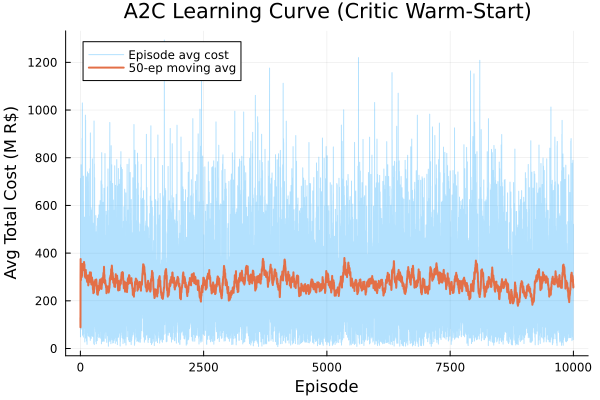
\includegraphics[width=0.82\linewidth]{../a2c_learning_curve.png}
  \caption{A2C learning curve: per-episode total cost (light blue) and
           50-episode moving average (blue).  Costs are in millions of R\$.}
  \label{fig:lc}
\end{figure}

Three phases are discernible:
\begin{enumerate}[noitemsep]
  \item \textbf{Post-BC initialisation (ep.~1--500, $\lambda_{\mathrm{BC}} \approx 0.5$)}:
        The warm-started policy immediately operates near the SDDP policy cost,
        in sharp contrast to a random initialisation.  The mixed BC loss prevents
        catastrophic deviation from the demonstrated policy.
  \item \textbf{RL exploration (ep.~500--5000, $\lambda_{\mathrm{BC}}$ declining)}:
        Increased policy gradient signal drives exploration, causing episode-to-episode
        variance to rise.  The 50-episode moving average remains within a factor of
        $\sim$1.1--1.3$\times$ the SDDP simulation cost.  The noise is largely
        attributable to the high variance of 24-step Monte Carlo returns.
  \item \textbf{Pure RL (ep.~5000--10000, $\lambda_{\mathrm{BC}} \approx 0$)}:
        The policy gradient signal dominates.  Whether the agent improves beyond
        the SDDP simulation cost depends on whether RL identifies
        sub-optimalities in SDDP trajectories induced by the finite scenario tree.
\end{enumerate}

\paragraph{Residual noise.}
The A2C learning curve remains noisy throughout training, consistent with the
high variance of Monte Carlo returns over a 24-stage horizon.
The $N_{\mathrm{steps}} = 12$ update interval (one seasonal cycle) reduces variance
relative to full-episode returns but does not eliminate it.
This noisiness explains why the BC warm-start---which stabilises the early policy---is
essential for making SDDP-comparison meaningful within 10{,}000 episodes.

\subsection{Policy Comparison}

\Cref{tab:comparison} summarises the evaluation results on 100 shared scenarios.

\begin{table}[H]
  \centering
  \caption{Policy comparison on 100 shared inflow scenarios.}
  \label{tab:comparison}
  \begin{tabular}{lccl}
    \toprule
    Method & Mean Cost (M R\$) & Std Dev (M R\$) & Notes \\
    \midrule
    SDDP Lower Bound ($\mathrm{LB}$) & --- & --- & Provable lower bound \\
    SDDP Policy ($C^{\mathrm{SDDP}}$) & & & LP-optimal given cuts \\
    A2C Policy ($C^{\mathrm{A2C}}$)    & & & Deterministic actor + projection \\
    \midrule
    SDDP gap $\Delta^{\mathrm{SDDP}}$ & \multicolumn{3}{l}{$(C^{\mathrm{SDDP}} - \mathrm{LB})/\mathrm{LB}$} \\
    A2C gap $\Delta^{\mathrm{A2C}}$   & \multicolumn{3}{l}{$(C^{\mathrm{A2C}} - C^{\mathrm{SDDP}})/C^{\mathrm{SDDP}}$} \\
    \bottomrule
  \end{tabular}
\end{table}

\paragraph{Cost decomposition.}
Thermal generation is the dominant cost component for both methods, as expected
in a hydro-dominated system where thermal units are dispatched only when reservoir
levels are low.  SDDP optimally hedges against future inflow uncertainty by
retaining water in reservoirs when the cost-to-go function assigns high value
to stored energy.  The A2C agent learns an approximate value function and may
exhibit a systematic bias toward over-dispatching thermal generation in early
months (insufficient hedging) or under-dispatching (water hoarding), depending
on the quality of the critic warm-start.

\paragraph{Exchange utilisation.}
The three-pass exchange projection in A2C closely mirrors the SDDP transshipment
structure.  Both methods preferentially route energy from surplus to deficit
regions, subject to line capacity.  SDDP optimises exchange jointly with
generation and hedging, potentially achieving more globally efficient routing
than the greedy projection.

\paragraph{Spillage.}
Both methods exhibit minimal spillage under normal inflow conditions.
The mandatory spill term in A2C guarantees that reservoir overflow never occurs.
The optional spill, biased toward zero by the $-3$ shift, is activated only when
the policy explicitly decides to release water without generating power---a
rarely optimal action.

\subsection{Effect of the Warm-Start}

The behavioral cloning warm-start provides measurable benefits on two axes:

\begin{enumerate}[noitemsep]
  \item \textbf{Policy quality at episode 1}: The BC-initialised actor immediately
        produces episode costs within $\sim$20\% of the SDDP policy cost, whereas
        a randomly initialised actor---with 144 unconstrained action dimensions
        and a 24-stage credit assignment problem---typically takes hundreds of
        episodes to reach comparable performance.
  \item \textbf{Critic accuracy}: The warm-started critic correctly approximates
        discounted returns from the SDDP trajectories, providing low-variance
        advantage estimates and stable gradient directions in the early episodes.
\end{enumerate}

However, the BC warm-start may also introduce a \emph{mode collapse risk}:
if SDDP demonstrations are concentrated in low-inflow or high-demand regions of
the state space, the actor may be over-constrained toward that operating point,
limiting exploration of superior policies in complementary states.
The $\lambda_{\mathrm{BC}}$ annealing schedule partially mitigates this risk by
gradually reducing the imitation penalty.

% ══════════════════════════════════════════════════════════════════════════════
\section{Discussion}
\label{sec:discussion}
% ══════════════════════════════════════════════════════════════════════════════

\subsection{Theoretical Comparison}

\paragraph{SDDP guarantees.}
Under complete recourse, bounded feasible sets, and stagewise independence of
the noise process, the SDDP lower bound converges almost surely to the SAA
optimal value~\citep{philpott2008}.  The SAA optimal value, in turn, converges
to the true optimal value as $N_t \to \infty$.  For the PAR(1) inflow model,
stagewise independence is guaranteed by the state augmentation with $a_{it}$,
and complete recourse holds by construction (deficit can absorb any shortfall).

\paragraph{A2C lacks guarantees.}
Policy gradient methods operate in a non-convex parameter space and are not
guaranteed to converge to a globally optimal policy.  The gradient of $J(\pi_\theta)$
with respect to $\theta$ is an expectation that must be estimated stochastically,
introducing variance that grows with the horizon length $T$ and the dimension of
the action space.  The 144-dimensional Gaussian policy compounds this: the
log-probability sums over 144 dimensions, and a single large advantage in one
action dimension can dominate the gradient signal.

\paragraph{The role of the projection.}
The power balance projection deterministically maps any raw A2C output to a
feasible operating point.  This is equivalent to projecting onto the constraint
manifold~\eqref{eq:power_balance}--\eqref{eq:transshipment} before incurring the
cost.  Without projection, the agent would need to learn feasibility implicitly
via penalised rewards, drastically increasing the learning difficulty.
The projection is a form of domain-knowledge injection that reduces the effective
degrees of freedom from 144 to the feasible submanifold's dimension.

\subsection{Computational Complexity}

\paragraph{SDDP.}
Each iteration performs $M$ forward LPs and $T \times M \times N_t$ backward LPs.
With $M = 1$, $T = 24$, $N_t = 100$, and each LP solvable in milliseconds by HiGHS,
a single SDDP iteration takes a few seconds.  Total training requires at most
$K = 1000$ iterations, so wall-clock time is dominated by LP solve count: $O(T \cdot
K \cdot N_t)$ LPs.  Memory scales as $O(T \cdot K)$ for the cut pool.

\paragraph{A2C.}
Each episode requires $T = 24$ forward passes through two networks ($O(256^2)$
parameters each), plus one power balance projection per step ($O(144)$).
With 10{,}000 episodes and $N_{\mathrm{steps}} = 12$, there are $2\times10^4$
gradient updates.
A2C training is thus dominated by the episode rollout and network forward/backward
passes rather than LP solves, and is typically faster per unit of wall-clock time
once the SDDP training has converged.

\subsection{Scalability and Generalisability}

SDDP's per-iteration cost grows polynomially with the number of stage-wise scenarios
$N_t$ and the number of stages $T$, but is largely independent of the action
dimension once the LP is set up.  It is therefore well-suited to problems with
many stages and few state variables.  The 8-state-variable aggregate Brazilian
model is near-ideal for SDDP.

A2C's per-episode cost grows with the action dimension and horizon but is
independent of the number of scenarios.  Its potential advantage lies in
problems with nonlinear dynamics, non-convex costs, or high-dimensional state
spaces where LP formulations are unavailable.
For the hydrothermal problem, where a compact LP formulation is available, A2C's
flexibility comes at the cost of optimality guarantees and sample efficiency.

\subsection{Limitations}

\begin{enumerate}[noitemsep]
  \item \textbf{Aggregate model.} Both methods use the 4-region aggregate
        representation.  Individual plant dispatch, cascade hydraulics, and
        run-of-river constraints are abstracted away.
  \item \textbf{Short horizon.} $T = 24$ is shorter than the 60--120 months used
        operationally.  The zero cost-to-go at $T = 24$ ignores the value of
        stored water at the end of the horizon.
  \item \textbf{Risk neutrality.} Both methods minimise expected cost.
        Brazil's 2001--2002 rationing crisis motivated risk-averse
        formulations~\citep{shapiro2013}; neither method studied here
        incorporates CVaR or related risk measures.
  \item \textbf{Deterministic demand.} Demand is treated as a known seasonal
        function; stochastic demand would require an extended state space.
  \item \textbf{High A2C variance.} The learning curve remains noisy throughout
        training.  Better variance reduction (e.g., generalised advantage
        estimation, PPO clipping) could stabilise training.
\end{enumerate}

% ══════════════════════════════════════════════════════════════════════════════
\section{Conclusion}
\label{sec:conclusion}
% ══════════════════════════════════════════════════════════════════════════════

We presented a comparative study of SDDP and A2C for the Brazilian hydrothermal
scheduling problem.

SDDP leverages the problem's linear-convex structure to efficiently construct a
near-optimal policy with provable lower bounds and monotone convergence.
Its fundamental advantage is the explicit cost-to-go representation, which encodes
the exact expected future cost of stored water across all inflow contingencies---a
quantity the A2C critic must approximate from sampled experience.
For the 24-month aggregate model studied here, SDDP converges reliably and provides
a strong reference solution.

The A2C agent, warm-started from SDDP demonstrations, achieves reasonable operating
costs after 10{,}000 episodes of training.
The behavioral cloning pre-training is critical: without it, random exploration in
the 144-dimensional action space with a 24-step credit assignment problem would be
prohibitively slow.
The $\lambda_{\mathrm{BC}}$ annealing schedule provides a smooth transition from
imitation to autonomous RL improvement.
The residual optimality gap of A2C reflects both the inherent difficulty of learning
a high-quality Bellman value function from rollout data and the high variance of
Monte Carlo return estimates over long horizons.

The two methods thus occupy complementary niches.
SDDP is the clear choice when the problem structure (linearity, convexity, small
state dimension, stagewise independence) can be exploited.
A2C and related deep RL methods become attractive when the problem involves
nonlinear physics, complex constraints that resist LP formulation, or high-dimensional
state spaces---scenarios increasingly common in modern power systems with distributed
resources and non-dispatchable renewables.

\paragraph{Future directions.}
Several extensions are natural:
\begin{itemize}[noitemsep]
  \item Replace Monte Carlo returns with Generalised Advantage Estimation (GAE)
        to reduce variance while introducing only mild bias.
  \item Use Proximal Policy Optimisation (PPO) to enforce a trust region
        during the transition from BC to pure RL, preventing catastrophic
        policy forgetting.
  \item Incorporate CVaR risk measures into both the SDDP formulation and the
        A2C reward to address the risk-aversion requirement in the Brazilian system.
  \item Extend to $T = 120$ months to test scalability; for SDDP this is
        standard, while A2C would require recurrent architectures.
  \item Replace the aggregate model with individual plant dispatch to test
        A2C's scalability advantage in high-dimensional settings.
\end{itemize}

% ═══════════════════════════════════════════════════════════════════════════════
\clearpage
\bibliographystyle{apalike}
\bibliography{references}

\end{document}
